\chapter{联邦学习的安全聚合模型}
\label{ch4}

上一章节中我们提出的方案是针对本地差分隐私,在我们的威胁模型中,对手可能是一个用户或者第三方,并且对手还可能是除其他用户和第三方外的中心服务器,这是一个相当强的威胁模型假设,因为除了用户本身,所有对象都是不可信的,用户在上传信息时需要经过满足差分隐私的噪声扰动。然而,强大的隐私也带来了模型可用性的问题,特别是当用户的数据量特别小时,聚合所有用户的参数会带来大量的噪声,从而降低了模型的精度。

在梯度上传至参数服务器前,隐私保护方案会对梯度添加噪声,尽管方案采用了本地差分技术减少一定程度的隐私预算,但不可避免的会降低联邦学习模型的准确性以及学习效率。正如\cite{ref37}所指出的,一个复杂的隐私保护系统将多个局部差异化的算法进行组合,从而导致这些算法的隐私成本的构成。也就是说,隐私预算为ε1和ε2的局部差异化算法的组合会消耗隐私预算为ε1+ε2。使用联合学习训练DNN需要客户在多次迭代中向云上传梯度更新。如果在迭代训练过程中的每一次迭代都应用 LDP,隐私预算就会累积起来,从而导致总隐私预算的爆炸。现有的本地差分隐私协议对于多维聚集FL可能是不可行的。这是因为局部噪声带来的误差会随着维度系数的增加而加剧\cite{ref38}。此外,由于参与一次迭代的客户端数量通常为几千人,会导致聚合升级为一个高维任务。

因此在这一小节中,论文提出一种信任域机制应用在分布式联邦学习协议中。我们将信任域与本地差分隐私相结合,用来提高在满足差分隐私保护后的联邦学习的模型精度。在本章节中我们提出了一个在联邦学习中的安全SA模型,本地数据使用本地差分隐私进行加密,然后所有人传到一个安全混洗器,安全混洗器打乱次序,再发给分析器(不包含任何标识信息)。安全混洗器可以作为一个可信第三方,独立于服务器并专门用于安全混洗器。安全SA模型的精度增益来自于隐私放大效应\cite{ref39},这表明本地随机器的洗牌(即匿名)输出在差分隐私的中心视图中比没有洗牌器的输出提供更强的(放大的)隐私。因此,在洗牌模型中需要更少的本地噪音,以获得对不信任的分析器的相同水平的隐私。我们将会在本章节详细的描述该框架中各个模块的设计和实现过程。


\section{问题定义}
\subsection{攻击模型}
攻击模型以一种新的方式使用生成对抗网络。在分布式联邦学习系统框架中,我们将生成对抗网络用于从正常参与者的协作学习中提取隐私信息,生成对抗网络生成一些应该只在被攻击参与者本地训练的训练集样本。基于GAN的方法在联邦学习的训练阶段有效,攻击者以白盒方式访问其余参与者模型,可以得到模型的内部参数。因为联邦学习协议的目的就是共享参数,这让攻击者执行成员推理攻击时,不需要考虑只能查询每个特定输入与模型输出的黑盒模式。 

在 GAN 攻击模型中,攻击方案并不是让攻击者自己完成GAN网络的对抗训练,而是利用生成对抗网络的思想,将本地的生成器网络和全局的神经网络进行对抗训练。在描述该部分攻击模型时,论文将分布式联邦学习系统简化为两个用户,一个为攻击者 A,一个为被攻击者 V,他们在系统中共享模型和参数。在简化模型中,被攻击者V有着一定量的训练集样本,对深度学习网络进行本地训练,上传模型参数。攻击者A 在本地也有一些正常的训练样本,引导被攻击者 V 尽可能多次数的上传参数。 


\section{安全框架}
该框架主要由编码器(encoder)、混洗器(shuffler)和分析器(analyzer)3部分组成:编码器运行在客户端,对用户数据进行本地化的编码、分割、扰动等处理;混洗器运行在一个半诚信的第三方,它可借助现有的安全混洗协议\cite{ref40}\cite{ref41}\cite{ref42}\cite{ref43}\cite{ref44}\cite{ref45}\cite{ref46}在对数据一无所知的情况下完成安全的混洗操作;分析器运行在真正的数据收集者端,对收集的数据进行校正与分析.该框架中,混洗器完成了对用户数据完全匿名的操作,使得用户可以在尽可能对数据本身进行较小扰动的情况,获得较多的隐私保护. 

\subsection{Shuffle 模型}
SA框架的协议由三个部分组成:$\mathcal{P}=\mathcal{A} \circ \mathcal{S} \circ \mathcal{R}^{n}$,$\mathcal{A}$表示分析器,$\mathcal{S}$表示Suffler,$\mathcal{R}^{n}$表示n个用户的数据集。如图\ref{fig:shuffle模型}所示。每个用户持有一维数据$x \in \mathbb{X}$,我们将n个用户的数据表示为数据集$X=\left(x_{1}, \cdots, x_{n}\right) \in \mathbb{X}^{n}$,每个用户运行一个随机器$\mathcal{R}: \mathbb{X} \rightarrow \mathbb{Y}^{m}$,将本地数据扰乱成满足$epsilon_{l}$-DP的信息。我们重点讨论$m=1$的单消息协议。 Shuffler执行$\mathcal{S}: \mathbb{Y}^{*} \rightarrow \mathbb{Y}^{*}$,用均匀随机的扰动 $pi$对收到的消息进行处理。分析器函数$\mathcal{A}: \mathbb{Y}^{*} \rightarrow \mathbb{Z}$ 将shuffle后的消息作为输入,并输出分析结果。

\begin{figure}[!hbt]
\centering
  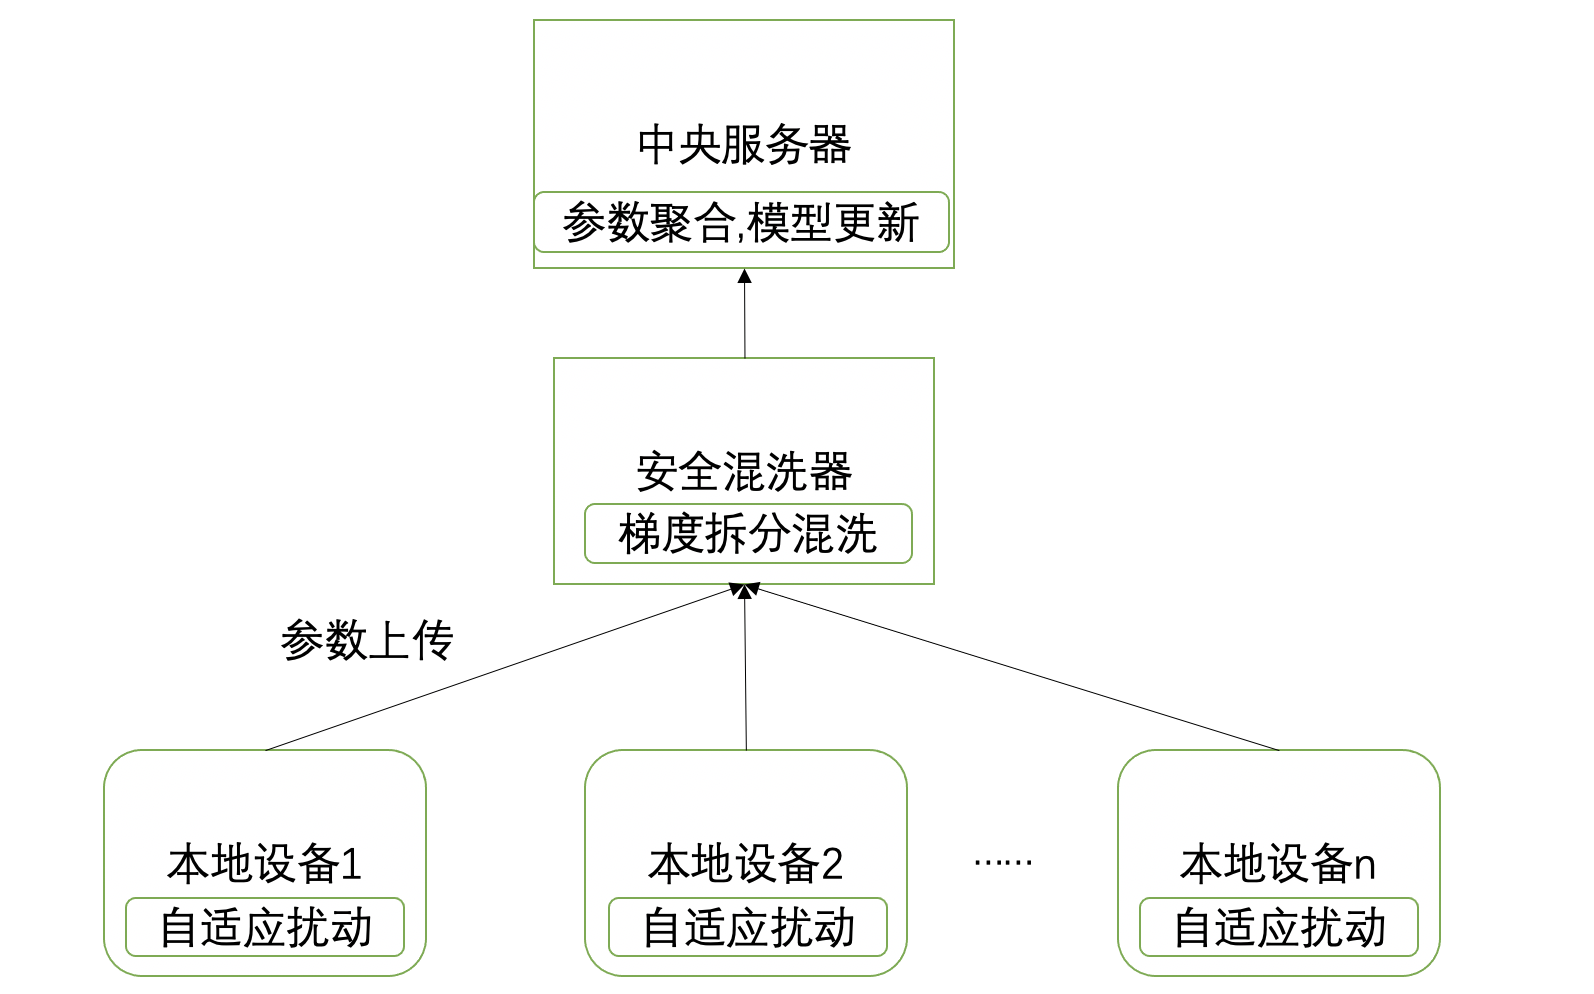
\includegraphics[scale=0.4]{fig2/C4/shuffle模型}%联邦学习的系统架构
  \caption{安全shuffle模型}
  \label{fig:shuffle模型} 
\end{figure}

\textbf{客户端参与方}:
假设有n个客户端参与房,每个参与房拥有一个$d$-维的局部更新向量$x_{i}$,参照第三章的本地差分操作进行扰动,得到模型的输出$y_{i}$。

\textbf{混洗器}:
混洗器是安全聚合的中心服务器,从各个客户端收到的模型输出参数进行混洗,然后发送给分析器。混洗器是独立的半诚信(semi-honest)服务器,可在对数据内容一无所知的情况下执行安全的混洗操作,是ESA框架的核心组件。它的作用是接收用户编码后的数据,消除相应的元数据(包括接收时间、顺序、IP地址等),并对接收数据进行混洗(即打乱顺序),以达到匿名目的.为保证足够的隐私保护效果,该混洗器需等待一段时间收集足够的用户数据进行混洗,并对数据量满足一定阈值的数据进行发布.当数据量为敏感信息时,可对该阈值添加满足差分隐私的噪声进行扰动,或者随机丢掉一些数据使数据量满足差分隐私\cite{ref47},从而保护数据量隐私。

\textbf{分析器$\mathcal{A}$}:
分析器$\mathcal{A}$从混洗器拿到安全聚合后的参数并对均方差进行估计,并更新全局模型。分析器由数据收集者运行,是不可信服务器.它的作用是接收混洗器发布的数据,依据相应的编码和混洗规则对数据进行分析与校正,并获取最终的统计结果.该框架中数据的隐私性主要是针对分析器而言的,即将分析器视为数据的窥探者. 


SA模型中的隐私目标是确保$\mathcal{M}=\mathcal{S} \circ \mathcal{R}^{n}$ 满足 $\left(\epsilon_{c}, \delta_{c}\right)-\mathrm{DP}$,因为$\mathcal{A}$是由一个不受信任的分析器执行,他没有义务保护用户的隐私。协议$\mathcal{P}$实现了与$mathcal{M}$相同的隐私水平。因此,我们重点分析$\mathcal{M}(X)$和$\mathcal{M}\left(X^{\prime}\right)$的不可区分性。Erlingsson等人2019年证明,$\mathcal{M}$的隐私可以被 "放大"。换句话说,当每个用户应用$\mathcal{R}$中的局部隐私预算$epsilon_{l}$时,$\mathcal{M}$可以实现$\left(\epsilon_{c}, \delta_{c}\right)-\mathrm{DP}$-DP的更强隐私性,当$\epsilon_{c}<\epsilon_{l}$时。与本地模型相比,洗牌模型需要更少的噪声来达到相同的隐私水平。

使用算法\ref{shuffle algorithm}中的局部随机器$\mathcal{R}_{\gamma, b}$ ,其中$\gamma=\frac{b}{e^{\epsilon} l+b-1}$表示从空白分布中输出一个元素的概率,输入值$x$被编码到一个离散域$[b]$,然后进行随机化。在$\mathcal{S}$运行了一次置换后,$\mathcal{A}$汇总洗牌结果 $\hat{z} \leftarrow \frac{1}{b} \sum_{i=i}^{n} y_{i}$ 并用以下方法进行去偏差:
\begin{equation}\label{eq:shuffle去偏差}
z \leftarrow(\hat{z}-n \gamma / 2) /(1-\gamma)
\end{equation}

\begin{algorithm}[!htb]
  \caption{安全混洗算法}
  \label{shuffle algorithm}
  \begin{algorithmic}[1]
    \footnotesize
    \STATE \textbf{Input:} scalar $x \in[0,1]$
    \STATE \textbf{Output:} perturbed value $y \in[b]$
      \STATE $\bar{x} \leftarrow\lfloor x b\rfloor+\operatorname{Ber}(x b-\lfloor x b\rfloor)$
      \STATE Sample $r \leftarrow \operatorname{Ber}(\gamma)$
      \STATE $y=\left\{\begin{array}{ll}\bar{x} & \text { if } r=0 \\ \operatorname{Unif}(\{1, \cdots, b\}) & \text { else. }\end{array}\right.$
    \STATE end
  \end{algorithmic}
\end{algorithm}

\subsection{信任边界}
我们把观察者表示为$\mathcal{O}$,它可以是任何可以观察全局模型参数的好奇者。在分布式差分隐私的联邦学习模型中中,隐私边界与$\mathcal{O}$和$\mathcal{A}$相关。而在本地差分隐私的联邦学习模型中,隐私边界在每个个体用户和其他成员之间。通过引入Shuffler $\mathcal{S}$,避免了像DP-FL那样将全部信任放在任何一方,同时能够实现比LDP-FL更好的模型效用。

我们设计了一个细粒度的隐私分离方案,并与表格中的DP-FL和LDP-FL进行比较。具体来说,我们将每个本地更新的信息分为:索引、相应的值和用户身份(即图2中的ID)。应该注意的是,当索引被选择并以取决于值的方式发送到shuffler $\mathcal{S}$时,它们可能是敏感的。因此,我们的隐私目标是以数据无关的方式选择索引,梯度的真实值对$\mathcal{S}$来说是不可见的。但$\mathcal{S}$应该知道用户的隐性身份,以便分发全局模型参数和接收本地上传的信息。对于观察者$\mathcal{O}$来说,$\left(\epsilon_{c}, \delta_{c}\right)-\mathrm{DP}$通过后处理属性而成立\cite{ref47},Shuffler处理后的信息不会暴露用户身份,并且满足针对A的$\left(\epsilon_{c}, \delta_{c}\right)-\mathrm{DP}$。在LDP-FL中,每个用户都需要一个$\left(\epsilon_{c}, \delta_{c}\right)-\mathrm{LDP}$ $\mathcal{R}$来实现这一目标。

\section{方案设计}
联邦学习的安全shuffle有三个构建过程:编码$\epsilon_{c}$,混洗 $\mathcal{S}$和中央服务器 $\mathcal{Z}$。在第8行,$\mathcal{C}$是矢量的剪切阈值。我们用$\epsilon_{l}$表示每个本地向量的本地隐私预算。$p k_{a}$和$s k_{a}$分别代表中央服务器产生的公钥和秘钥。下面的不同协议是通过实现第10行的Randomize $(\cdot)$和第15行的Shuffle $(\cdot)$函数,以不同的策略设计的。需要注意的是,算法1中的$\mathcal{R}_{\gamma, b}$可以作为基本随机器应用于Randomize $(\cdot)$中,这与行(18)的方程(1)的估计相吻合。也可以应用通用的随机器(例如拉普拉斯机制),这并不影响我们后面的推论。

\subsection{安全性假设}
我们假设洗牌者和分析者没有勾结(否则,模型会简化为LDP-FL)。我们还假设加密原语是安全的,并且对手在计算上很难从密码文本中获得任何信息。

\subsection{Shuffle协议}
\begin{algorithm}[!htb]
  \caption{Shuffle框架}
  \label{Shuffle框架}
  \begin{algorithmic}[1]
    \footnotesize
    \STATE \textbf{Input:} $\mathcal{A}, \mathcal{S}, \mathcal{E}, n, T, \epsilon_{l}, p k_{a}, s k_{a}$
    \STATE \textbf{Output:} $\theta^{T}$
      \STATE 中央服务器 $mathcal{Z}$中央服务器公开公钥$p k_{a}$
        \FOR{$t=1, \cdots, T$}
          \STATE $x_{i} \leftarrow$ LocalUpdate $\left(\theta^{t-1}\right)$
          \STATE 每个本地用户通过编码器$\epsilon_{c}$编码
          \STATE $\bar{x}_{i} \leftarrow \operatorname{Clip}\left(x_{i},-C, C\right)$
          \STATE $\tilde{x}_{i} \leftarrow\left(\bar{x}_{i}+C\right) /(2 C)$
          \STATE $\left\langle i d x_{i}, y_{i}\right\rangle \leftarrow$ Randomize $\left(\tilde{x}_{i}, \epsilon_{l}\right)$
          \STATE $c_{i} \leftarrow \operatorname{Enc}_{p k_{a}}\left(y_{i}\right)$
          \STATE 本地用户将$m_{i}=\left\langle i d x_{i}, c_{i}\right\rangle$发送给Shuffler
        \ENDFOR
      \STATE Shuffle
      \STATE Shuffle将混洗后的信息Shuffle $\left(m_{i \in[n]}\right)$发送给中央服务器
      \STATE 中央服务器
      \STATE 解密消息 $y_{\pi(i) \in[n]} \leftarrow \operatorname{Dec}_{s k_{a}}\left(c_{\pi(i) \in[n]}\right)$
      \STATE 计算均方差 $\bar{z} \leftarrow \frac{1}{n} \sum_{i \in[n]}\left\langle i d x_{i}, y_{i}\right\rangle$
      \STATE 求均值 $z \leftarrow C \cdot(2 \bar{z}-1)$
      \STATE 更新全局模型 $\theta^{t} \leftarrow \theta^{t-1}+z$
  \end{algorithmic}
\end{algorithm}

我们首先提出Shuffle协议:P = A ◦S ◦Rn,用于Shuffle框架下的d维聚合。简而言之,我们扩展了一维协议,对每个维度进行其随机化和聚集。根据差分隐私的组成属性,R应该满足$\epsilon_{l d^{-}}$LDP,其中$\epsilon_{l d}=\epsilon_{l} / d$。我们在\ref{Shuffle框架}中声明一个Randomize $(\cdot)$,当$i d x_{i} \leftarrow\{1, \cdots, d\}$,并且$y_{i} \leftarrow$ $\left\{\mathcal{R}_{\epsilon_{l d}}\left(x_{i, 1}\right), \cdots, \mathcal{R}_{\epsilon_{l d}}\left(x_{i, d}\right)\right\} .$。函数Shuffle $(\cdot)$简单地生成一个排列组合π,并输出m$m_{\pi(i) \in[n]}$。
然后我们针对中央服务器的DP后的信息进行核算。对$\mathcal{R}_{\gamma, b}$ 或其他通用$\mathcal{R}$的数值评估采取$\epsilon_{l d}$应用到Lemma 1,可以得出一个放大的中央隐私$\left(\epsilon_{c d}, \delta_{c d}\right)$。有了Lemma 3中的构成,我们可以很容易地推导出定理1中的向量级构成。推论2提炼了从$\epsilon_{l}$ 到 $\epsilon_{c}$的放大作用。

因此,相对于求和操作,缩放后的更新的灵敏度由S限制。GM现在将噪声(缩放至灵敏度S)添加到所有缩放后的更新之和。 将GM的输出除以mt可以得出所有客户更新的真实平均值的近似值,同时可以防止泄露有关个人的重要信息。

通过将此近似值添加到当前的中央模型wt中,可以分配新的中央模型wt + 1:
\begin{equation}
w_{t+1}=w_{t}+\frac{1}{m_{t}}(\underbrace{\overbrace{\sum_{k=0}^{m_{t}} \Delta w^{k} / \max \left(1, \frac{\left\|\Delta w^{k}\right\|_{2}}{S}\right)}^{\text {Sum of updates clipped at } S}}_{\text {Gaussian mechanism approximating sum of updates }})^{\text {Noise scaled to } S}
\end{equation}


当将1 / mt 分解为高斯机制时,我们注意到平均值的失真由噪声方差S2σ2/ m决定。但是,这种失真不应超过某个限制。否则,来自二次采样平均值的太多信息会被添加的噪声破坏,并且不会有任何学习进度。 GM和随机子采样都是随机机制。 (实际上,\cite{ref48}正是在dp-SGD中使用了这种平均逼近。但是,它用于梯度平均,在每次迭代时都隐藏单个数据点的梯度)。因此,σ和m还定义了随机机制提供平均近似值时所引起的隐私损失。

为了跟踪这种隐私损失,我们利用了Abadi等人提出的时刻会计\cite{ref49}。与标准组成定理相比,这种会计方法对发生的隐私损失提供了更严格的限制。策展人每次分配新模型时,会计都会根据ǫ,σ和m评估δ。一旦δ达到某个阈值,即客户贡献被透露的可能性变得过高,培训应停止。 δ阈值的选择取决于客户K的总数。要确定不保留许多人的隐私,而要以泄露一些人的全部信息为代价,我们必须确保δ≪ K1。

选择S:削减贡献时,需要权衡取舍。一方面,应选择较小的S,以使噪声方差保持较小。另一方面,一个人想保持尽可能多的原始贡献。按照\cite{ref50}提出的程序,在每个通信回合中,我们计算所有未裁剪贡献的中位数范数,并将其用作裁剪界限$S=$ median $\{\triangle w k\} k \in Z t$。我们不使用随机机制来计算中位数,严格来说,这是对隐私的侵犯。但是,通过中位数的信息泄漏很小(未来的工作将包含这种隐私措施)。

选择σ和m:对于固定的S,比率r=σ2/m控制失真和隐私损失。因此,σ越高,m越小,隐私损失就越大。隐私权会计师告诉我们,对于固定的r =σ2/m,即,对于相同的失真水平,对于σ和m都较小的隐私权损失较小。因此,失真率r的上限和子采样客户数m的下限将导致σ的选择。但是,很难估计m的下限。也就是说,因为联合设置中的数据是非IID,并且来自客户端的贡献可能非常不同。因此,我们将客户之间的差异Vc定义为客户更新之间相似度的量度。

\subsection{隐私性证明}
因为稀疏向量技术在隐私预算方面的潜在节省,本文选择将应用稀疏向量技术的差分隐私与应用选择梯度上传的分布式联邦学习协议相结合,达到更好的隐私保护效果。在应用稀疏向量技术时,我们对算法中有关输出向量阈值的选择与分布式联邦学习协议中的选择梯度上传阈值优化为同一步骤。为了保证经过这一修改后的算法仍然满足差分隐私,将在这一节对论文使用的方案是否满足差分隐私进行进一步的数学推
导证明。 

\begin{proof}
证明:基于安全shuffle的联邦学习随机梯度上传满足差分隐私。

考虑任意输出向量$a \in\{T, 1\}^{\ell}$,$a_{i}$表示 $a$ 的第 $\mathrm{i}$ 个组成部分。 $I_{T}=\left\{i: a_{i}=\mathrm{T}\right\}$ 表示查询的结果高于阈值的个数, $I_{\perp}=\left\{i: a_{i}=\mathbf{1}\right\}$, 表示查询的结果低于阈值的个数, 参数的敏感度不超过 $\Delta$; 隐私参数稀疏最大值 $c$, 差分隐私保护隐私预算 $\epsilon$。

可以得到梯度的 $\operatorname{Pr}[A(W)=a$ ]概率:

\begin{equation}
\begin{array}{l}
\operatorname{Pr}[A(W)=a]=\int_{-\infty}^{+\infty} \operatorname{Pr}[\rho=z] \prod_{i \in I_{T}} \operatorname{Pr}\left[q_{i}(W)+v_{i} \geq \boldsymbol{T}_{i}+z\right. \\
\prod_{i \in I_{\perp}} \operatorname{Pr}\left[q_{i}(W)+v_{i}<\boldsymbol{T}_{i}+z\right] d z
\end{array}
\end{equation}

对于梯度 $W$ 和保护后的梯度 $W^{\prime}$, 可以得到:

\begin{equation}
\begin{aligned}
\frac{\operatorname{Pr}[A(W)=a]}{\operatorname{Pr}\left[A\left(W^{\prime}\right)=a\right]} &=\frac{\int_{-\infty}^{+\infty} \operatorname{Pr}[\rho=z] \prod_{i \in l_{\top}} \operatorname{Pr}\left[q_{i}(W)+v_{i} \geq \boldsymbol{T}_{i}+z\right] d z}{\int_{-\infty}^{+\infty} \operatorname{Pr}[\rho=z] \Pi_{i \in I_{T}} \operatorname{Pr}\left[q_{i}\left(W^{\prime}\right)+v_{i} \geq \boldsymbol{T}_{i}+z\right] d z} \\
& \times \frac{\int_{-\infty}^{+\infty} \operatorname{Pr}[\rho=z] \prod_{i \in I_{\perp}} \operatorname{Pr}\left[q_{i}(W)+v_{i}<\boldsymbol{T}_{i}+z\right] d z}{\prod_{i \in I_{\perp}} \operatorname{Pr}\left[q_{i}\left(W^{\prime}\right)+v_{i}<\boldsymbol{T}_{i}+z\right] d z}
\end{aligned}
\end{equation}

设

\begin{equation}
\begin{array}{l}
f_{i}(W, z)=\operatorname{Pr}\left[q_{i}(W) v_{i}<\boldsymbol{T}_{i}+z\right] \\
g_{i}(W, z)=\operatorname{Pr}\left[q_{i}(W) v_{i} \geq \boldsymbol{T}_{i}+z\right]
\end{array}
\end{equation}

可以得到:
$$
\frac{\operatorname{Pr}[A(W)=a]}{\operatorname{Pr}\left[A\left(W^{\prime}\right)=a\right]}$$
$$=\frac{ \left.\int_{-\infty}^{+\infty} \operatorname{Pr}[\rho=z] \prod_{i \in I_{T}} g_{i}(W, z) \prod_{i \in I_{\perp}} f_{i}(W, z)\right] d z}{ \left.\int_{-\infty}^{+\infty} \operatorname{Pr}[\rho=z] \prod_{i \in I_{\top}} g_{i}\left(W^{\prime}, z\right) \prod_{i \in I_{\perp}} f_{i}\left(W^{\prime}, z\right)\right] d z}$$
$$=\frac{ \left.\int_{-\infty}^{+\infty} \operatorname{Pr}[\rho=z-\Delta] \prod_{i \in I_{T}} g_{i}(W, z-\Delta) \prod_{i \in I_{\perp}} f_{i}(W, z-\Delta)\right] d z}{ \left.\int_{-\infty}^{+\infty} \operatorname{Pr}[\rho=z] \prod_{i \in I_{\top}} g_{i}\left(W^{\prime}, z\right) \prod_{i \in I_{\perp}} f_{i}\left(W^{\prime}, z\right)\right] d z}$$
$$\leq \frac{ \left.\int_{-\infty}^{+\infty} e^{\epsilon_{1}} \operatorname{Pr}[\rho=z] \prod_{i \in I_{\perp}} f_{i}\left(W^{\prime}, z\right) \prod_{i \in I_{\mathrm{T}}} g_{i}(W, z-\Delta)\right] d z}{ \left.\int_{-\infty}^{+\infty} \operatorname{Pr}[\rho=z] \prod_{i \in I_{\perp}} f_{i}\left(W^{\prime}, z\right) \prod_{i \in I_{T}} g_{i}\left(W^{\prime}, z\right)\right] d z}$$
$$\leq \frac{ \left.\int_{-\infty}^{+\infty} e^{\epsilon_{1}} \operatorname{Pr}[\rho=z] \prod_{i \in I_{\perp}} f_{i}\left(W^{\prime}, z\right) \prod_{i \in l_{T}} e^{\frac{\epsilon_{\Omega}}{c}} g_{i}\left(W^{\prime}, z\right)\right] d z}{ \left.\int_{-\infty}^{+\infty} \operatorname{Pr}[\rho=z] \prod_{i \in I_{\perp}} f_{i}\left(W^{\prime}, z\right) \prod_{i \in I_{\top}} g_{i}\left(W^{\prime}, z\right)\right] d z}$$
$$\leq e^{\epsilon_{1}}\left(e^{\frac{\epsilon_{\Omega}}{c}}\right)^{c}=e^{\epsilon_{1}+\epsilon_{1}}=e^{\epsilon}$$
\end{proof}

根据上述推导证明可知, 基于安全shuffle的联邦学习随机梯度上传满足差分隐私, 所上传的梯度是满足 $\left(\epsilon_{1}+\epsilon_{2}\right)$-差分隐私的。

\section{本章总结}
本章针对第三章所提的联邦学习自适应本地差分机制为提出了基于信任域的优化方案。结合联邦系统参与者共享参数时选择梯度上传的规则,优化参数上传的阈值选择,在分布式联邦学习系统中设计更优的差分隐私保护方案。通过合理的参数选择,降低方案复杂度,对每部分上传的梯度进行差分保护,使分布式联邦学习系统达到隐私保护的效果。在此基础上,将信任域群保护和差分隐私保护方法结合在分布式系统中,在隐私保护协议下提高系统的整体性能。实验评估了差分隐私的保护效果,合理的参数选择才能够平衡数据隐私性和模型效率。




























